We are using Qt for Python(PySide2) for the NeXus Constructor's graphical user interface. These are the official bindings for Qt 5 C++ API, provided by the Qt company. 
\bigskip
There are two main methods of using Qt in Python, the more common "Widgets" framework or Qt-Quick which uses a markup language called QML.
We are taking the Qt-Widgets approach to developing the NeXus constructor, as the tooling for Qt-Quick/QML seems to be a bit lacking and some of the bindings are not pythonic, and rather use C++-like idioms. Widgets also look more native to the OS running them. 
\bigskip
Since version 5.12 PySide2 has included the Qt3D module in Qt5. We are utilising this with our 3d View of components in the neutron experiments. Qt3D provides a high-level interface to OpenGL which allows us to display the geometry information of components as well as an animated pulsed neutron beam.
\bigskip
\begin{figure}
\caption{Qt3D's element inspector}
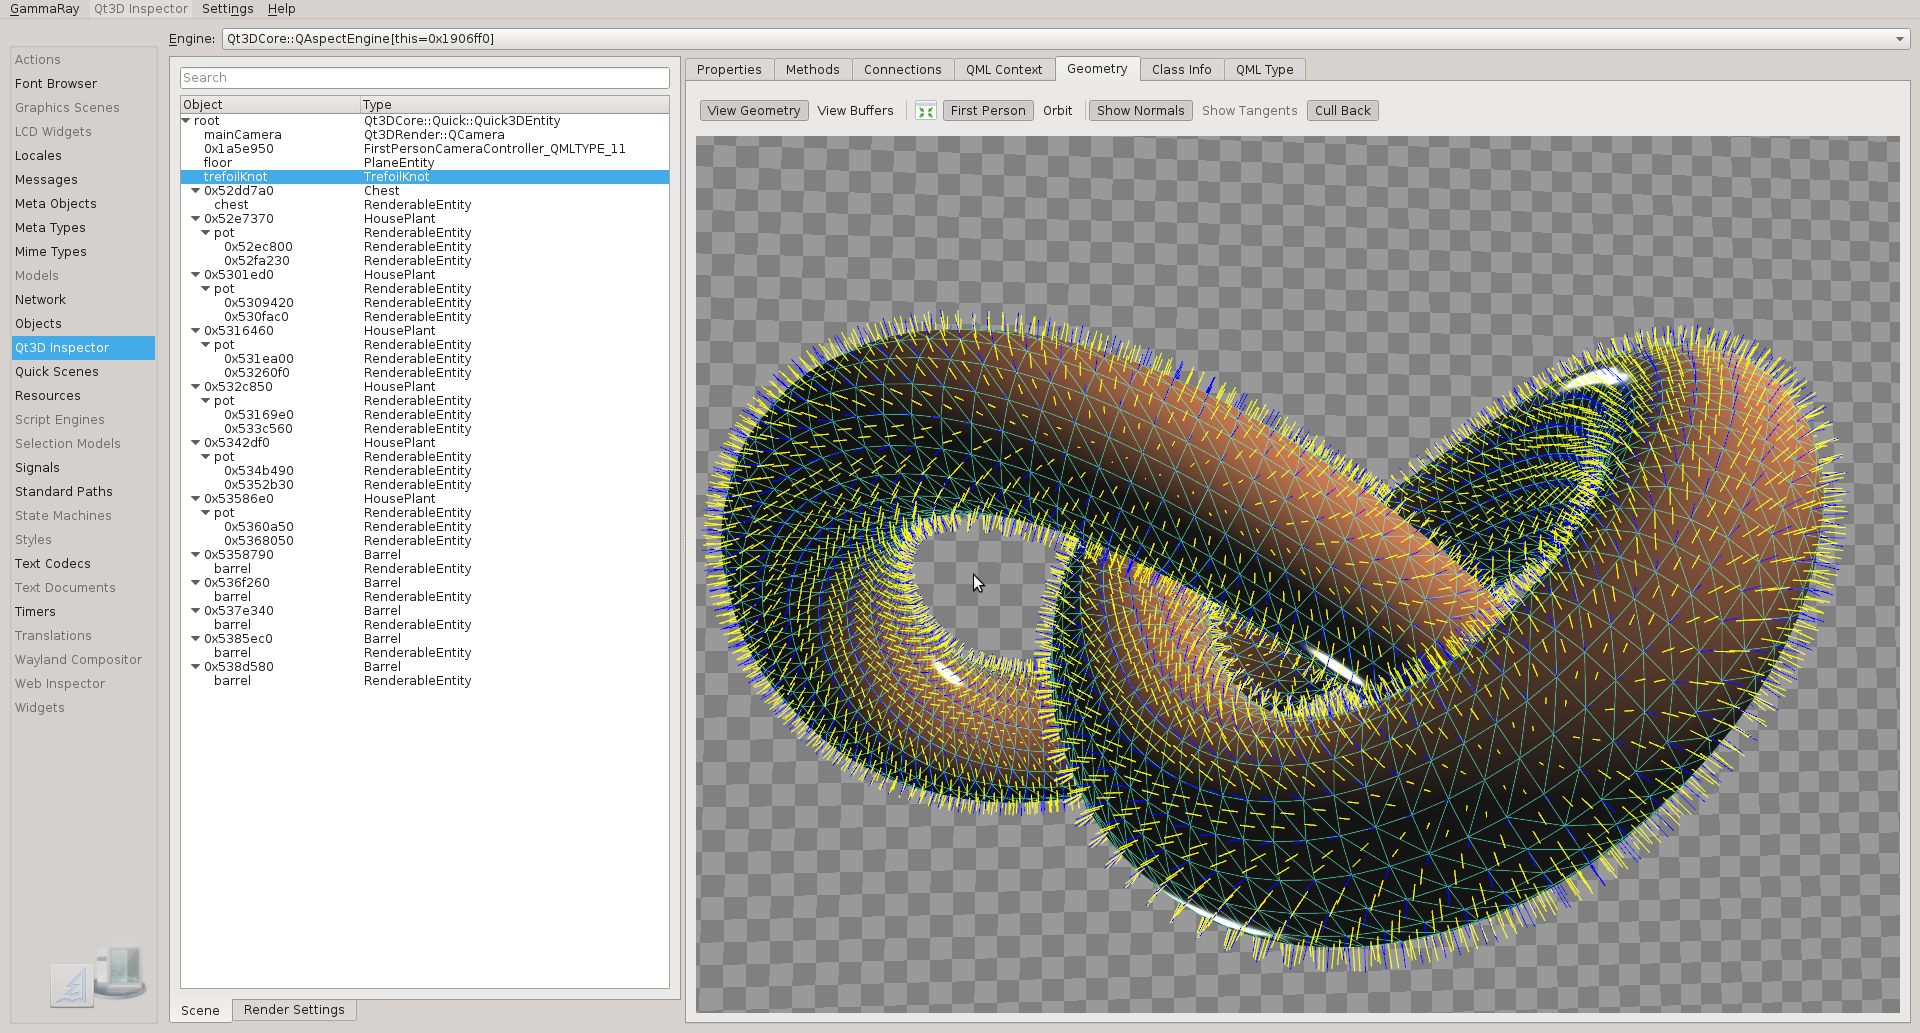
\includegraphics[width=\linewidth]{qt3d.png}
\end{figure}
\bigskip
